\block[]
{Here is some serious part}
{
\setlength{\columnsep}{30pt}
\begin{multicols*}{2}
{
    Lorem ipsum dolor sit amet, consectetur adipiscing elit, sed do eiusmod tempor incididunt ut labore et dolore magna aliqua. Eget nunc lobortis mattis aliquam. Id semper risus in hendrerit gravida. Adipiscing tristique risus nec feugiat in. Amet facilisis magna etiam tempor orci. Scelerisque viverra mauris in aliquam sem fringilla ut morbi tincidunt. Sit amet nisl suscipit adipiscing.\\
    Consectetur adipiscing elit ut aliquam purus sit. In est ante in nibh mauris cursus mattis. Auctor urna nunc id cursus metus aliquam eleifend. Egestas sed tempus urna et pharetra pharetra massa massa ultricies. Pulvinar pellentesque habitant morbi tristique senectus. Urna nunc id cursus metus aliquam. Urna molestie at elementum eu facilisis sed. Habitasse platea dictumst vestibulum rhoncus.
}
\pagebreak
{
    \coloredbox[bgcolor=gray, fgcolor=white, framecolor=colorFive, width=0.5\colwidth-45pt]{Leo in vitae turpis massa. Morbi tristique senectus et netus et malesuada fames. Adipiscing elit ut aliquam purus sit amet luctus venenatis lectus.}
    Congue quisque egestas diam in arcu cursus. Curabitur gravida arcu ac tortor dignissim. Dictum fusce ut placerat orci nulla pellentesque dignissim enim sit. Arcu risus quis varius quam quisque id diam vel. Aenean pharetra magna ac placerat vestibulum lectus mauris. Lectus quam id leo in vitae turpis massa. Tortor at auctor urna nunc id cursus metus aliquam eleifend. Nibh mauris cursus mattis molestie a iaculis at.
}
\end{multicols*}
}

\block[]
{The final part}
{
\setlength{\columnsep}{30pt}
\begin{multicols*}{2}
{
    \begin{tikzfigure}[Caption of the figure]
    \label{fig:fig1}
     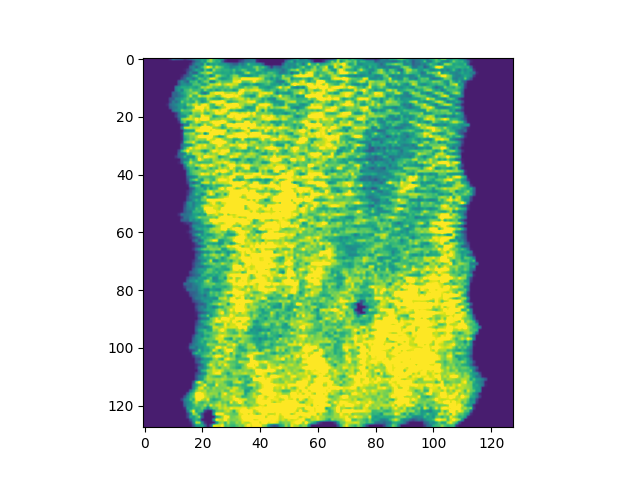
\includegraphics[width=0.5\colwidth-75pt]{Figure/7100_0.png}
    \end{tikzfigure}
}
\pagebreak
{
\begin{tikztable}[Summary Statistics for the 10 dimensional case of PSO 2007 with a ring neighborhood of 4. I know you don't know what it means\cite{C02}. But at least you have an example of a table. More info here \url{https://www.overleaf.com/learn/latex/Tables}]
    \begin{tabular}{llllll}
        D10 & min      & max      & std      & average  \\
        f1  & 0.00E+00 & 0.00E+00 & 0.00E+00 & 0.00E+00 \\
        f3  & 4.40E-02 & 1.37E+08 & 2.18E+07 & 6.46E+06 \\
        f8  & 2.01E+01 & 2.05E+01 & 8.44E-02 & 2.03E+01 \\
    \end{tabular}
\end{tikztable}

\vspace{5pt}

Nulla facilisi etiam dignissim diam quis enim lobortis scelerisque fermentum. Aliquam purus sit amet luctus venenatis lectus. Tincidunt tortor aliquam nulla facilisi. Porta lorem mollis aliquam ut porttitor leo. Cursus mattis molestie a iaculis at erat pellentesque adipiscing\cite{C03}.
}
\end{multicols*}
    % \end{tikzfigure}
}

\block[]
{Acknowledgements}
{
Thanks to my cat, love him! Also thanks to my father, my mother, my brother and sister, super happy to be here with everyone. Also thanks to this random guy who walked on my right feet this morning, super nice...
}

\block[]
{References}
{
% \setlength{\columnsep}{30pt}
% \begin{multicols*}{2}
    \printbibliography[heading=none]
% \end{multicols*}
}

